\documentclass[11pt,a4paper]{article}
\usepackage[T1]{fontenc}
\usepackage[margin=2.3cm]{geometry}
\usepackage{amsmath,amssymb}
\usepackage{graphicx}
\usepackage[dvipsnames]{xcolor}
\usepackage{enumitem}
\usepackage[colorlinks=true,linkcolor=blue,urlcolor=blue]{hyperref}
\setlength{\parskip}{0.6em}
\setlength{\parindent}{0pt}
\begin{document}

\begin{center}{\LARGE\bfseries openneuron}\\[0.4em]{\large Simulate a nerve cell firing, and how its signal travels, in three sessions.}\\[0.2em]\small PAN IIT OSS explainer \textbullet{} secondary school to diploma / undergraduate (levels 3-5)\end{center}

\section*{Why this exists}
Nerve cells communicate with brief electrical pulses. This explainer follows the idea from a simple threshold, through the membrane as a resistor and capacitor, to the Hodgkin-Huxley equations of the squid giant axon, using only simple differential equations that you can solve numerically yourself. It is general education, not medical information.

\section*{The end goal}
Simulate a nerve cell firing and how signals travel. The end goal is to simulate a nerve cell firing and to understand how the signal travels: where the threshold comes from, why every spike looks the same, what limits the firing rate and why fibre diameter, insulation and temperature change the speed.

\section*{How the three sessions build up}
\begin{enumerate}[nosep]
\item \textbf{Session 1: A neuron adds up signals and fires a spike} (Level 1, conceptual interactive model, 60 min).
\item \textbf{Session 2: The membrane is an RC circuit: the leaky integrate-and-fire neuron} (Level 2, mathematical engineering model, 75 min).
\item \textbf{Session 3: The Hodgkin-Huxley nerve: a simulation you can validate} (Level 3, simulation and validation, 90 min).
\end{enumerate}

\section{Session 1: A neuron adds up signals and fires a spike}

\subsection*{A. Real-world problem}
Every thought, touch and movement is carried by nerve cells that talk with brief electrical pulses called spikes. A neuron receives signals from other cells on its branches (dendrites), adds them up in its cell body, and, if the total voltage crosses a threshold, fires one spike that runs down its long wire (the axon). A faint touch makes few spikes and a hard push makes many, but every spike looks the same. How can a cell turn a smooth input into this on-off signal? This repo is general education only: it shows a simplified model, not medical information.

\subsection*{B. Concept and theory}
We model the voltage V inside the cell relative to the outside, in millivolts (mV). At rest it sits at V\_rest = -70 mV (a typical textbook value). Each millisecond the input pushes V up by the drive d (mV per ms) and a leak pulls it back towards rest by a fraction k = 0.1 of the distance. If the drive is constant, V settles at V\_rest + d / k. A threshold V\_th = -55 mV decides firing: when V reaches it, the neuron fires a spike of fixed height, V resets to rest, and a refractory time of 2 ms follows during which it cannot fire again. A constant drive can fire the neuron only if the settling level lies above the threshold, which means d \textgreater{} k (V\_th - V\_rest) = 1.5 mV per ms. After the spike starts, it travels along the axon at a roughly constant speed v, so the delay over a length L is L / v.

\begin{itemize}[nosep]
\item V: membrane voltage (inside minus outside) (mV)
\item V\_rest: resting voltage, typical -70 (mV)
\item V\_th: threshold voltage, typical -55 (mV)
\item d: drive: push added to V each millisecond (mV per ms)
\item k: leak fraction per millisecond (0.1) (per ms)
\item L, v: axon length and spike speed (m, m per s)
\end{itemize}

\begin{equation*}
V_{n+1}=V_n+d-k\,(V_n-V_{\mathrm{rest}})
\end{equation*}

\begin{equation*}
V_\infty=V_{\mathrm{rest}}+\frac{d}{k},\qquad d_{\min}=k\,(V_{\mathrm{th}}-V_{\mathrm{rest}})
\end{equation*}

\begin{equation*}
\Delta t=\frac{L}{v}
\end{equation*}

\begin{center}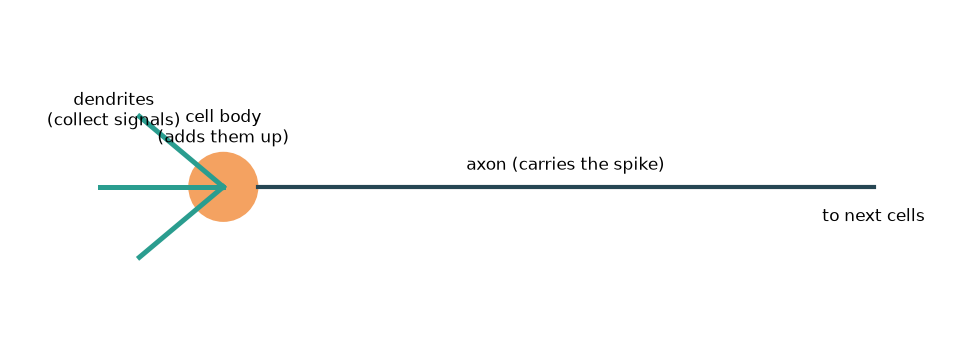
\includegraphics[width=0.85\linewidth]{figures/s01_neuron_picture.png}\\\small A neuron: dendrites collect signals, the cell body adds them up, the axon carries the spike.\end{center}

\subsection*{E. Worked example}
A constant drive of 2.0 mV per ms is applied from rest. Will the neuron fire, and after how many milliseconds?
\begin{enumerate}[nosep]
\item Settling level: V\_inf = -70 + 2.0 / 0.1 = -50 mV. That is above the threshold of -55 mV, so it will fire.
\item With the drive constant the climb is V(n) = -70 + 20 (1 - 0.9\textasciicircum{}n). We need V(n) = -55, which means 20 (1 - 0.9\textasciicircum{}n) = 15 and so 0.9\textasciicircum{}n = 0.25.
\item n = ln 0.25 / ln 0.9 = 13.16 steps, so 13 steps are not enough and 14 are.
\item Check: V(13) = -55.08 mV (just below the threshold) and V(14) = -54.58 mV (above it), so the first spike comes at step 14, that is 14 ms.
\item The simulation agrees: the first spike is at 14 ms and there are 6 spikes in 100 ms.
\end{enumerate}
\textbf{Answer.} Yes. The first spike comes at 14 ms (13.16 steps rounded up), and the neuron fires 6 times in 100 ms.

\subsection*{F. Questions}
\begin{enumerate}[nosep]
\item \textbf{Conceptual.} A stronger stimulus does not make a bigger spike. So how does a nerve tell the brain that a touch is stronger?
\item \textbf{Numerical.} For a constant drive of 3.0 mV per ms find the level the voltage would settle at, and the step at which the first spike happens (hand calculation, then check with the code).
\item \textbf{Graph and simulation interpretation.} In the trace for drive 1.0 mV per ms the voltage rises and then flattens out below the threshold line. What level does it flatten at, and why is there no spike?
\item \textbf{Design and optimisation challenge.} Design: a model neuron must fire at least 10 times in 100 ms, and a spike must cross a 0.5 m axon in under 5 ms. Choose a drive (in steps of 0.5 mV per ms) and an axon speed, and say what trade-off you see.
\end{enumerate}

\section{Session 2: The membrane is an RC circuit: the leaky integrate-and-fire neuron}

\subsection*{A. Real-world problem}
The membrane of a nerve cell keeps charge apart, so it stores energy like a capacitor C, and ion channels let charge leak through like a resistor R. If we inject a current I the voltage obeys C dV/dt = -(V - V\_rest)/R + I. Add the rule 'when V reaches the threshold, record a spike, reset V and wait a refractory time' and you have the leaky integrate-and-fire (LIF) neuron. How fast does it fire for a given current? And what current makes it fire exactly 20 times a second? (General education only; the numbers are typical textbook values, not measurements of a particular cell.)

\subsection*{B. Concept and theory}
Charge conservation gives C dV/dt = -(V - V\_rest)/R + I: the current that does not leak away charges the capacitor. For a constant I the exact solution is V(t) = V\_rest + R I (1 - exp(-t / tau)) with tau = R C: the voltage climbs towards V\_rest + R I and covers 63.2 percent of the climb in one tau. Units: 1 megaohm times 1 nanoamp is 1 mV, and 1 megaohm times 1 pF is 1 microsecond, so with R in megaohm and C in pF, tau in ms is R C / 1000. Typical values R = 100 megaohm and C = 100 pF give tau = 10 ms. The voltage can reach the threshold V\_th = -55 mV only if R I \textgreater{} V\_th - V\_rest = 15 mV, so the rheobase is I = 15 mV / R = 0.15 nA. Setting V(T) = V\_th and solving gives the climb time T = tau ln(R I / (R I - 15 mV)). With the reset at V\_rest = -70 mV and a refractory time t\_ref = 2 ms, one cycle lasts t\_ref + T and the rate is f = 1 / (t\_ref + T); with t\_ref = 0 it is the closed form f = 1 / (tau ln(R I / (R I - (V\_th - V\_rest)))). Typical numbers used here: V\_rest = -70 mV, V\_th = -55 mV, V\_reset = -70 mV.

\begin{itemize}[nosep]
\item V: membrane voltage (mV)
\item C: membrane capacitance, typical 100 (pF)
\item R: membrane (leak) resistance, typical 100 (megaohm)
\item I: injected current (nA)
\item tau: time constant R C, typical 10 (ms)
\item V\_rest, V\_th, V\_reset: rest, threshold and reset voltages, typical -70, -55, -70 (mV)
\item t\_ref: refractory period, typical 2 (ms)
\item f: firing rate (spikes per second (Hz))
\end{itemize}

\begin{equation*}
C\,\frac{dV}{dt}=-\frac{V-V_{\mathrm{rest}}}{R}+I
\end{equation*}

\begin{equation*}
V(t)=V_{\mathrm{rest}}+R I\left(1-e^{-t/\tau}\right),\qquad \tau=RC
\end{equation*}

\begin{equation*}
I_{\mathrm{rheo}}=\frac{V_{\mathrm{th}}-V_{\mathrm{rest}}}{R}
\end{equation*}

\begin{equation*}
T=\tau\ln\frac{R I}{R I-(V_{\mathrm{th}}-V_{\mathrm{rest}})},\qquad f=\frac{1}{t_{\mathrm{ref}}+T}
\end{equation*}

\begin{center}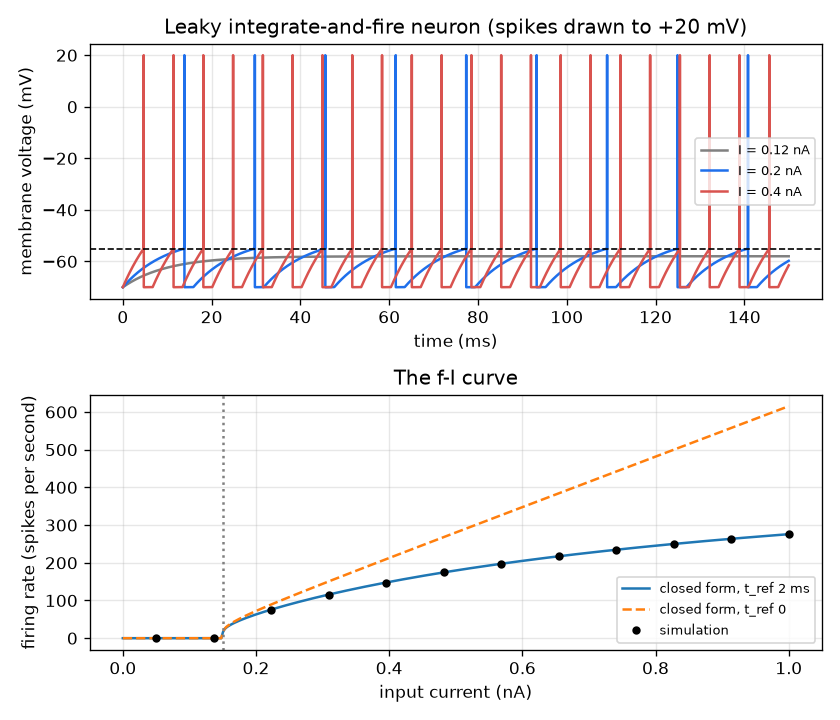
\includegraphics[width=0.85\linewidth]{figures/s02_lif_and_fi.png}\\\small Top: LIF voltage traces for three currents. Bottom: the f-I curve, closed form against simulation.\end{center}

\subsection*{E. Worked example}
For R = 100 megaohm, C = 100 pF and I = 0.2 nA, find the time to reach the threshold and the firing rate with t\_ref = 2 ms.
\begin{enumerate}[nosep]
\item tau = R C = 100 x 100 / 1000 = 10 ms. R I = 100 x 0.2 = 20 mV, which is above the 15 mV needed, so it fires.
\item T = tau ln(R I / (R I - 15)) = 10 ln(20 / 5) = 10 ln 4 = 13.863 ms.
\item One cycle = 2 + 13.863 = 15.863 ms, so f = 1000 / 15.863 = 63.04 spikes per second.
\item Without a refractory period the rate would be 1000 / 13.863 = 72.13 per second.
\item Simulation check: the numerical spike train has its first spike at 13.87 ms and every interval is 15.87 ms.
\end{enumerate}
\textbf{Answer.} T = 13.863 ms and f = 63.04 spikes per second (72.13 without the refractory period).

\subsection*{F. Questions}
\begin{enumerate}[nosep]
\item \textbf{Conceptual.} If R stays the same but the capacitance C is halved, does the neuron fire faster or slower for the same current? Explain without equations, then check with a number.
\item \textbf{Numerical.} For R = 100 megaohm, C = 100 pF and I = 0.3 nA find the climb time T and the rate f (t\_ref = 2 ms).
\item \textbf{Graph and simulation interpretation.} Describe the shape of the f-I curve: what happens below 0.15 nA, just above it, and for very large currents? What does the limit mean?
\item \textbf{Design and optimisation challenge.} Design: the cell must fire at 20 spikes per second, within 18 to 22. Find the current for exactly 20 per second, the allowed range of current, and say what makes this design delicate.
\end{enumerate}

\section{Session 3: The Hodgkin-Huxley nerve: a simulation you can validate}

\subsection*{A. Real-world problem}
The leaky integrate-and-fire neuron of Session 2 draws the spike by hand. A real nerve cell builds its spike from the physics of ion channels: sodium channels open and let positive charge rush in, then they close and potassium channels open and let charge flow out. In 1952 Hodgkin and Huxley wrote four coupled equations for the squid giant axon that reproduce the spike, the threshold, the refractory period and repetitive firing. Can you integrate them yourself, trust the result, and find out how fast the cell can fire and what makes the signal faster? (General education only: a classic textbook model of one axon, not a medical tool.)

\subsection*{B. Concept and theory}
We use the modern sign convention: V is inside minus outside, rest is near -65 mV, and a depolarisation is a rise of V. The membrane obeys a current balance per unit area with three ion currents: sodium g\_Na m\textasciicircum{}3 h (V - E\_Na), potassium g\_K n\textasciicircum{}4 (V - E\_K) and a leak g\_L (V - E\_L). The gates m, h and n are probabilities between 0 and 1 that relax towards values set by the voltage: dx/dt = alpha\_x(V) (1 - x) - beta\_x(V) x for x = m, h, n, where alpha and beta are the standard empirical rate functions of Hodgkin and Huxley (listed in the lesson, in 1/ms). Classic squid-axon parameters at 6.3 C: C = 1 uF/cm\textasciicircum{}2, g\_Na = 120, g\_K = 36, g\_L = 0.3 mS/cm\textasciicircum{}2, E\_Na = 50, E\_K = -77, E\_L = -54.387 mV (the leak reversal is chosen so that rest is -65 mV; in the original 1952 convention V is measured from rest with the opposite sign, E\_L = 10.6 mV). Temperature enters through the Q10 idea: all gate rates are multiplied by Q10\textasciicircum{}((T - 6.3)/10) with Q10 = 3. Axon diameter enters through cable theory: the length constant is lambda = sqrt(r\_m / r\_i), r\_i is proportional to 1/a\textasciicircum{}2 and r\_m to 1/a for radius a, so lambda grows as sqrt(a) and the speed scales as sqrt(a) (a scaling argument, tested below with a cable simulation). Numerics: RK4 takes four slope estimates per step; it is stable only for steps small compared with the fastest time scale of the model.

\begin{itemize}[nosep]
\item V: membrane voltage (inside minus outside) (mV)
\item m, h, n: sodium activation, sodium inactivation, potassium activation gates (0 to 1)
\item C: membrane capacitance per area, 1 (uF/cm\textasciicircum{}2)
\item g\_Na, g\_K, g\_L: maximum sodium and potassium conductances and the leak, 120, 36, 0.3 (mS/cm\textasciicircum{}2)
\item E\_Na, E\_K, E\_L: reversal potentials 50, -77, -54.387 (mV)
\item I\_ext: applied current per area (uA/cm\textasciicircum{}2)
\item alpha, beta: gate opening and closing rates (1/ms)
\item Q10, T: rate multiplier per 10 C (3) and temperature (no unit, C)
\item a, v: axon radius and conduction speed (um, m/s)
\end{itemize}

\begin{equation*}
C\frac{dV}{dt}=I_{\mathrm{ext}}-g_{\mathrm{Na}}m^3h\,(V-E_{\mathrm{Na}})-g_{\mathrm{K}}n^4\,(V-E_{\mathrm{K}})-g_{\mathrm{L}}\,(V-E_{\mathrm{L}})
\end{equation*}

\begin{equation*}
\frac{dx}{dt}=\alpha_x(V)\,(1-x)-\beta_x(V)\,x,\qquad x\in\{m,h,n\}
\end{equation*}

\begin{equation*}
\alpha_m=\frac{0.1\,(V+40)}{1-e^{-(V+40)/10}},\quad \beta_m=4e^{-(V+65)/18},\quad \alpha_h=0.07e^{-(V+65)/20},\quad \beta_h=\frac{1}{1+e^{-(V+35)/10}}
\end{equation*}

\begin{equation*}
\alpha_n=\frac{0.01\,(V+55)}{1-e^{-(V+55)/10}},\quad \beta_n=0.125\,e^{-(V+65)/80}
\end{equation*}

\begin{equation*}
V_{\mathrm{LIF}}(t)=V_{\mathrm{rest}}+\frac{I}{g_0}\left(1-e^{-g_0t/C}\right),\quad g_0=g_{\mathrm{Na}}m^3h+g_{\mathrm{K}}n^4+g_{\mathrm{L}}
\end{equation*}

\begin{equation*}
\lambda=\sqrt{r_m/r_i}\propto\sqrt{a}\ \Rightarrow\ v\propto\sqrt{a}
\end{equation*}

\begin{center}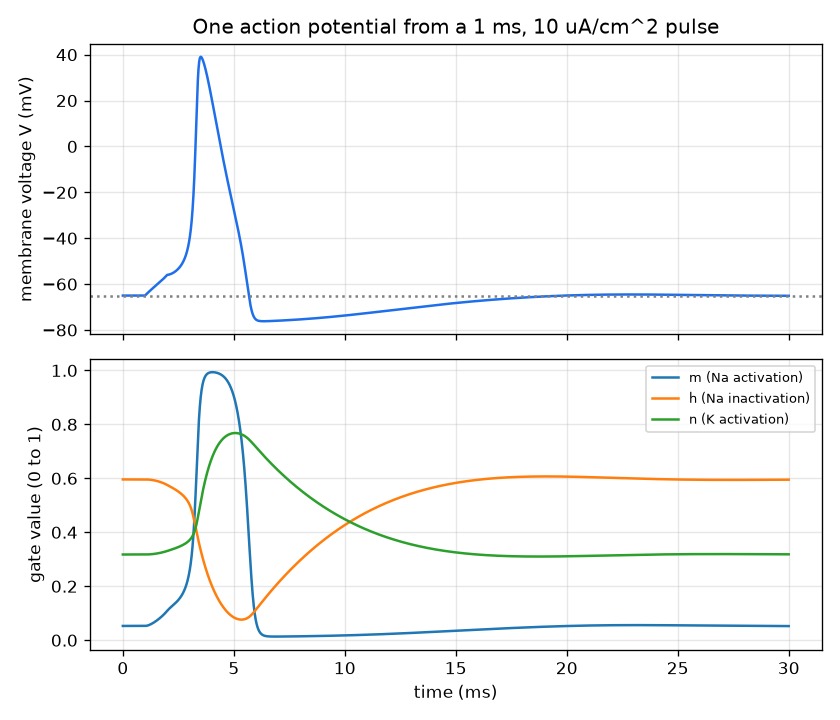
\includegraphics[width=0.85\linewidth]{figures/s03_action_potential.png}\\\small One action potential and the three gating variables: m rises first, h falls, n rises slowly.\end{center}

\subsection*{E. Worked example}
Find the smallest 1 ms pulse that fires a spike, and show that the spike is all or nothing.
\begin{enumerate}[nosep]
\item Integrate the four equations with RK4 (dt = 0.02 ms) from the resting state V = -65.0 mV, gates m = 0.053, h = 0.596, n = 0.318.
\item Apply a 1 ms pulse of amplitude A at t = 1 ms and bisect on A: the smallest amplitude that crosses 0 mV is 6.92 uA/cm\textasciicircum{}2.
\item A pulse of 6.5 uA/cm\textasciicircum{}2 peaks at only -59.1 mV and decays: no spike.
\item Pulses of 7.5, 15 and 30 uA/cm\textasciicircum{}2 all produce a spike peaking between 36 and 42 mV: the size of the spike does not follow the size of the pulse.
\item Cross-check with the charge: a 1 ms pulse of 6.92 uA/cm\textasciicircum{}2 delivers 6.92 nC/cm\textasciicircum{}2, which charges C = 1 uF/cm\textasciicircum{}2 by about 7 mV at once, enough to reach the threshold region from -65 mV.
\end{enumerate}
\textbf{Answer.} The threshold of a 1 ms pulse is 6.92 uA/cm\textasciicircum{}2; below it the voltage fades (peak -59.1 mV at 6.5), above it a full spike of about 40 mV appears whatever the strength.

\subsection*{F. Questions}
\begin{enumerate}[nosep]
\item \textbf{Conceptual.} Why does a spike appear suddenly once the stimulus passes a threshold, and why is it the same size for every stronger stimulus?
\item \textbf{Numerical.} For a tiny current of 0.1 uA/cm\textasciicircum{}2 the membrane acts, for the first moments, like a leaky capacitor with g\_0 = 0.6775 mS/cm\textasciicircum{}2. Calculate by hand the voltage rise after 0.2 ms and compare it with the simulation.
\item \textbf{Graph and simulation interpretation.} On the f-I curve, what happens at currents below 6.27, just above it, and at very large currents? What does this say about the cell?
\item \textbf{Design and optimisation challenge.} Design: a spike must travel 1 m in 20 ms, that is 50 m/s. Using the scaling v proportional to sqrt(a) and the simulated 7.97 m/s for a 100 um radius, what radius would an unmyelinated axon need? What does this suggest, and what temperature effect would you expect?
\end{enumerate}

\section{Real-world mini-project}
\textbf{Find the weakest stimulus and the fastest firing of a model nerve.} An experimenter wants two numbers from the Hodgkin-Huxley model with the classic squid-axon parameters at 6.3 C. First, the weakest stimulus that makes the cell fire: use \texttt{strength\_duration} from Session 3 to find the threshold current for pulses of 0.2, 1 and 50 ms, and the charge each carries. Second, the highest firing rate: use \texttt{max\_rate\_scan} over constant currents from 55 to 65 uA/cm\textasciicircum{}2.

\section{The path ahead}
\begin{enumerate}[nosep]
\item \textbf{Session 4: Up-and-down current sweep and a live f-I curve.} A simulation with a triangle current ramp (zero to 30 and back to zero uA/cm\textasciicircum{}2 over 2000 ms) whose f-I curve is built point by point, separately for the up and the down branch.
\item \textbf{Session 5: A stable integrator for large steps.} A solver that integrates the gating equations with the exact exponential update and V with a stable scheme.
\item \textbf{Session 6: Saltatory conduction in a myelinated axon.} A cable model with insulated segments and active nodes.
\item \textbf{Session 7: Two neurons joined by a synapse.} Two leaky integrate-and-fire neurons, the first driving the second.
\item \textbf{Session 8: Spike-frequency adaptation.} A leaky integrate-and-fire neuron with an adaptation variable.
\end{enumerate}

\section{Answers and hints}

\subsection*{Session 1}
\begin{enumerate}[nosep]
\item \textbf{Conceptual.} Hint: Compare the traces for weak, medium and strong drive: what changed, and what stayed the same? Solution: The spike height is fixed (all or nothing), but a stronger input pushes the voltage back to the threshold sooner after each spike, so the neuron fires more often. The strength is carried by the rate (and by how many neurons fire), not by the size of a spike. In the model the drive 2.0 gives 6 spikes in 100 ms and the drive 4.0 gives 14, all of the same height.
\item \textbf{Numerical.} Hint: Settling level = -70 + d / 0.1. The first spike needs 0.9\textasciicircum{}n = 1 - 15 (0.1) / d. Solution: Settling level = -70 + 3.0 / 0.1 = -40 mV, above the threshold. Then 0.9\textasciicircum{}n = 1 - 1.5 / 3.0 = 0.5, so n = ln 0.5 / ln 0.9 = 6.58, rounded up to step 7. The code gives the first spike at 7 ms. Unit check: the drive is in mV per ms, so d / k is in mV.
\item \textbf{Graph and simulation interpretation.} Hint: Use the settling level -70 + d / 0.1 and compare it with -55. Solution: It flattens at -70 + 1.0 / 0.1 = -60 mV, 5 mV below the threshold of -55 mV. The leak removes charge as fast as the drive adds it once V reaches -60, so the voltage never gets to -55 and there is no spike. Raising the drive to above 1.5 mV per ms moves the settling level above the threshold.
\item \textbf{Design and optimisation challenge.} Hint: Count the spikes for drive 2.5, 3.0 and 3.5 with the code; the delay is 1000 L / v in ms. Solution: Drive 2.5 gives 9 spikes (too few), drive 3.0 gives 11 spikes and drive 3.5 gives 12, so the smallest drive in steps of 0.5 that works is 3.0 mV per ms. The delay is 1000 (0.5) / v \textless{} 5 ms, so v must exceed 100 m/s (exactly 5 ms at 100 m/s). Trade-off: a larger drive costs more input but fires faster; a faster axon needs a thicker (or insulated) fibre, which takes more space and material. Assumption: constant drive and constant speed.
\end{enumerate}

\subsection*{Session 2}
\begin{enumerate}[nosep]
\item \textbf{Conceptual.} Hint: A smaller capacitor holds less charge for the same voltage, so it fills up (and reaches the threshold) sooner. tau = R C. Solution: Faster. The time constant tau = R C halves, so the voltage reaches the threshold sooner after every reset. Check with R I = 30 mV: for C = 100 pF the rate is 111.96 Hz, for C = 50 pF it is 182.96 Hz and for C = 200 pF it is 63.04 Hz. The threshold level (set by R I) does not change; only the speed of the climb does.
\item \textbf{Numerical.} Hint: R I = 30 mV. Use T = tau ln(R I / (R I - 15)). Solution: tau = 10 ms and R I = 30 mV. T = 10 ln(30 / 15) = 10 ln 2 = 6.931 ms. One cycle = 2 + 6.931 = 8.931 ms, so f = 1000 / 8.931 = 111.96 spikes per second. Sanity check: the current is twice the rheobase, and the rate is well above the 63 Hz found for 0.2 nA, as it should be.
\item \textbf{Graph and simulation interpretation.} Hint: Read the curve at 0.15, 0.16 and the far right of the graph. Solution: Below the rheobase of 0.15 nA the rate is zero. Just above it the rate jumps to a finite value (33.64 Hz at 0.16 nA), because the climb to the threshold becomes quick once R I exceeds 15 mV by even a little. For very large currents the climb time T goes to zero and the rate approaches 1 / t\_ref = 500 Hz (for a huge current of 1000 nA it is already 500 Hz to within 0.5). The refractory period sets the maximum rate.
\item \textbf{Design and optimisation challenge.} Hint: Invert the formula: T = 1000 / f - t\_ref and R I = 15 / (1 - exp(-T / tau)). Solution: For 20 per second the cycle is 50 ms, so T = 48 ms and R I = 15 / (1 - exp(-4.8)) = 15.12 mV, hence I = 0.1512 nA. For 18 per second I = 0.1507 nA and for 22 per second I = 0.1520 nA, so the allowed range is only about 0.0013 nA wide. The design is delicate because the target rate is close to the rheobase 0.15 nA, where the rate rises steeply with current: raising the current from 0.151 to 0.152 nA (less than 1 percent) raises the rate from 19.17 to 22.07 Hz. Real neurons are noisy, so a more robust design uses a current well above the rheobase and a higher rate.
\end{enumerate}

\subsection*{Session 3}
\begin{enumerate}[nosep]
\item \textbf{Conceptual.} Hint: Think about what happens to the sodium current as V rises, and about what ends the spike. Solution: Depolarisation opens sodium gates (m rises), which lets sodium flow in, which depolarises the cell further: positive feedback. Below the threshold the potassium and leak currents win and the voltage decays; above it the feedback runs away until V approaches E\_Na. The spike then ends by itself because h falls (sodium inactivates) and n rises (potassium opens). The peak is set by the channels, not by the stimulus, so every spike looks the same.
\item \textbf{Numerical.} Hint: V - V\_rest = (I / g\_0)(1 - exp(-g\_0 t / C)), with C = 1 uF/cm\textasciicircum{}2. Solution: I / g\_0 = 0.1 / 0.6775 = 0.1476 mV and g\_0 t / C = 0.6775 x 0.2 / 1 = 0.1355, so 1 - exp(-0.1355) = 0.1267 and the rise is 0.1476 x 0.1267 = 0.01870 mV. The HH simulation gives 0.01887 mV, within 1 percent. Units: (uA/cm\textasciicircum{}2) / (mS/cm\textasciicircum{}2) = mV. After 1 ms the gates have moved and HH is 11 percent above this leaky curve: the limit of the leaky model.
\item \textbf{Graph and simulation interpretation.} Hint: Compare the rates at 8, 10, 60 and 66 uA/cm\textasciicircum{}2. Solution: Between the rheobase (2.25 uA/cm\textasciicircum{}2) and 6.27 the cell fires exactly one spike and rests. At 6.27 sustained firing starts, and the rate jumps to about 60 Hz (62.5 Hz at 8 and 68.3 at 10 uA/cm\textasciicircum{}2), so it cannot fire slowly: the cell has no low-rate regime in this model. The rate rises to a maximum near 126 Hz (125.9 Hz at 63 uA/cm\textasciicircum{}2) and at 66 uA/cm\textasciicircum{}2 the cell stops firing repetitively (depolarisation block): too much current keeps sodium inactivated.
\item \textbf{Design and optimisation challenge.} Hint: v2 / v1 = sqrt(a2 / a1), so a2 = a1 (v2 / v1)\textasciicircum{}2. Solution: a2 = 100 um x (50 / 7.97)\textasciicircum{}2 = about 3936 um, a radius near 4 mm, which is huge: unmyelinated fibres can be fast only if they are thick. That is why animals that need fast signals use a different trick, myelin (not modelled here), instead of giant axons. Warm temperature speeds up all the gate rates (Q10 = 3 multiplies them by 3.8 between 6.3 and 18.5 C, and the spike width shrinks from 1.45 to 0.42 ms), so a warm axon is faster; we do not claim an exact speed factor, only the direction. The scaling is only an estimate of the trend.
\end{enumerate}

\section{How to join}
Read \texttt{CONTRIBUTING.md} in the repository, then pick an issue labelled \texttt{good first issue}. Repository: \url{https://github.com/KrunalPanchal1995/openneuron}

\end{document}
